\chapter{Выбор элементной базы}

\section{Выбор МШУ1}

Хорошим выбором входного усилителя будет \href{https://www.analog.com/en/products/hmc902lp3e.html}{HMC902LP3} производства Analog Devices.
Он обладает следующими характеристиками:
\begin{itemize}
    \item
        рабочий диапазон частот $(5 \ldots 11)~\text{ГГц}$;
    \item
        коэффициент усиления $K = 19.5~\text{дБ}$;
    \item
        коэффициент шума $NF = 1.8~\text{дБ}$;
    \item
        точка однодецибельной компрессии $P1dB = 16~\text{дБм}$;
    \item
        точка пересечения третьего порядка $IP3 = 28~\text{дБм}$.
\end{itemize}

Функциональная диаграмма HMC902LP3 приведена на Рис.~\ref{fig:hmc902lp3e_functional_diagram}.

\begin{figure}[!ht]
    \centering
    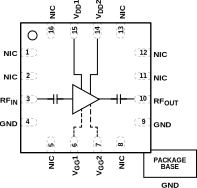
\includegraphics[width=0.4\textwidth]{hmc902lp3e_functional_diagram.pdf}
    \caption{Функциональная диаграмма усилителя HMC902LP3}%
    \label{fig:hmc902lp3e_functional_diagram}
\end{figure}

Частотные характеристики устройства приведены на Рис.~\ref{fig:hmc902lp3e_responses}.

\begin{figure}[!ht]
    \centering
    \begin{subfigure}[b]{0.45\textwidth}
        \centering
        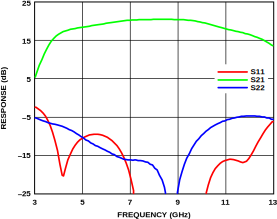
\includegraphics[width=\textwidth]{hmc902lp3e_response.pdf}
        \caption{}%
        \label{fig:hmc902lp3e_response}
    \end{subfigure}
    \hfill
    \begin{subfigure}[b]{0.45\textwidth}
        \centering
        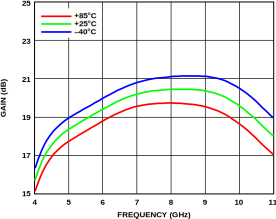
\includegraphics[width=\textwidth]{hmc902lp3e_gain.pdf}
        \caption{}%
        \label{fig:hmc902lp3e_gain}
    \end{subfigure}
    \caption{%
        Частотные характеристики:
        (а) усиление и коэффициенты отражения;
        (б) усиление при различных температурах
    }%
    \label{fig:hmc902lp3e_responses}
\end{figure}

Габариты устройства приведены на Рис.~\ref{fig:hmc902lp3e_outline_drawing}.
Стоит обратить внимание на размер выводов и расстояния между ними, т.к. цепи согласования будут проектироваться на основе этой информации.

\begin{figure}[!ht]
    \centering
    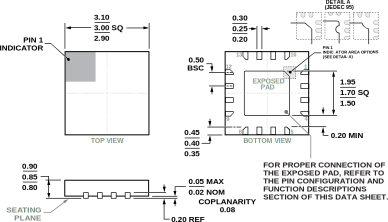
\includegraphics[width=0.8\textwidth]{hmc902lp3e_outline_drawing.pdf}
    \caption{Габариты усилителя HMC902LP3}%
    \label{fig:hmc902lp3e_outline_drawing}
\end{figure}

\section{Выбор МШУ2}

К выходному усилителю предъявляются не такие строгие требования по коэффициенту шума, поэтому, в связи с тем, что не было подходящего малошумящего усилителя с достаточным для удовлетворения техническому заданию усилением, было принято решение поставить обычный.

Хорошим выбором выходного усилителя будет \href{https://www.analog.com/en/products/hmc633lc4.html}{HMC633LC4} производства Analog Devices.
Он обладает следующими характеристиками:
\begin{itemize}
    \item
        рабочий диапазон частот $(5.5 \ldots 17)~\text{ГГц}$;
    \item
        коэффициент усиления $K = 30~\text{дБ}$;
    \item
        коэффициент шума $NF = 10~\text{дБ}$;
    \item
        точка однодецибельной компрессии $P1dB = 23~\text{дБм}$;
    \item
        точка пересечения третьего порядка $IP3 = 30~\text{дБм}$.
\end{itemize}

Функциональная диаграмма HMC633LC4 приведена на Рис.~\ref{fig:hmc633lc4_functional_diagram}.

\begin{figure}[!ht]
    \centering
    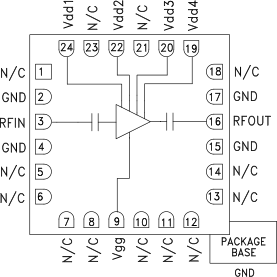
\includegraphics[width=0.4\textwidth]{hmc633lc4_functional_diagram.pdf}
    \caption{Функциональная диаграмма усилителя HMC633LC4}%
    \label{fig:hmc633lc4_functional_diagram}
\end{figure}

Частотные характеристики устройства приведены на Рис.~\ref{fig:hmc633lc4_responses}.

\begin{figure}[!ht]
    \centering
    \begin{subfigure}[b]{0.45\textwidth}
        \centering
        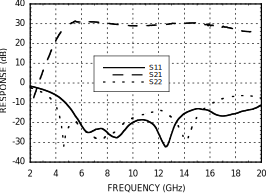
\includegraphics[width=\textwidth]{hmc633lc4_response.pdf}
        \caption{}%
        \label{fig:hmc633lc4_response}
    \end{subfigure}
    \hfill
    \begin{subfigure}[b]{0.45\textwidth}
        \centering
        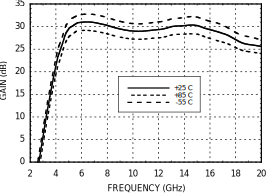
\includegraphics[width=\textwidth]{hmc633lc4_gain.pdf}
        \caption{}%
        \label{fig:hmc633lc4_gain}
    \end{subfigure}
    \caption{%
        Частотные характеристики:
        (а) усиление и коэффициенты отражения;
        (б) усиление при различных температурах
    }%
    \label{fig:hmc633lc4_responses}
\end{figure}

Габариты устройства приведены на Рис.~\ref{fig:hmc633lc4_outline_drawing}.
Стоит обратить внимание на размер выводов и расстояния между ними, т.к. цепи согласования будут проектироваться на основе этой информации.

\begin{figure}[!ht]
    \centering
    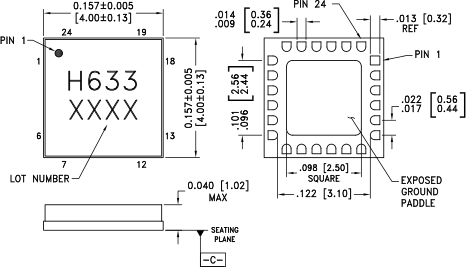
\includegraphics[width=0.8\textwidth]{hmc633lc4_outline_drawing.pdf}
    \caption{Габариты усилителя HMC633LC4}%
    \label{fig:hmc633lc4_outline_drawing}
\end{figure}

\section{Выбор фазовращателя}

Хорошим выбором фазовращателя будет \href{https://www.qorvo.com/products/p/TGP2105-SM}{TGP2105-SM} производства Qorvo.
Он обладает следующими характеристиками:
\begin{itemize}
    \item
        рабочий диапазон частот $(6 \ldots 18)~\text{ГГц}$;
    \item
        шаг фазы $LSB = 5.625^\circ$;
    \item
        точка однодецибельной компрессии $P1dB = 25~\text{дБм}$;
    \item
        точка пересечения третьего порядка $IP3 = 41~\text{дБм}$.
\end{itemize}

Функциональная диаграмма TGP2105-SM приведена на Рис.~\ref{fig:tgp2105sm_functional_diagram}.

\begin{figure}[!ht]
    \centering
    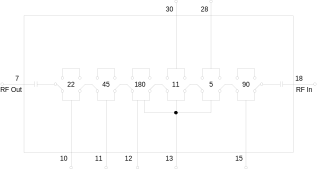
\includegraphics[width=0.8\textwidth]{tgp2105sm_functional_diagram.pdf}
    \caption{Функциональная диаграмма усилителя TGP2105-SM}%
    \label{fig:tgp2105sm_functional_diagram}
\end{figure}

Габариты устройства приведены на Рис.~\ref{fig:tgp2105sm_outline_drawing}.
Стоит обратить внимание на размер выводов и расстояния между ними, т.к. цепи согласования будут проектироваться на основе этой информации.

\begin{figure}[!ht]
    \centering
    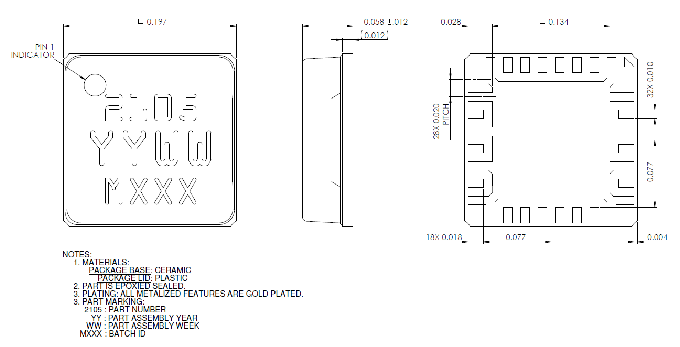
\includegraphics[width=0.8\textwidth]{tgp2105sm_outline_drawing.pdf}
    \caption{Габариты усилителя TGP2105-SM}%
    \label{fig:tgp2105sm_outline_drawing}
\end{figure}
